\begin{frame}[label=title]
    \centering
    \begin{figure}[H]
        
\includegraphics[keepaspectratio, width=0.7\paperwidth, height=\paperheight]{LeeLogo}
    \end{figure}
    Informatik: Data Science und Sicherheit\\
    \emoji{clamp}\textbf{Kompression}
\end{frame}

\begin{frame}{Weshalb Kompression? \emoji{clamp}}
	\begin{itemize}
		\item Speicherplatz optimieren
	\end{itemize}
	\begin{figure}[H]
		\centering
		
\includegraphics[width=.6\textwidth]{GrundlagenInfo/DataScience/04_Kompression/Figures/compression3}
	\end{figure}
	\begin{figure}[H]
		\centering
		\raisebox{-0.5\height}{
\includegraphics[width=.2\textwidth]{GrundlagenInfo/DataScience/04_Kompression/Figures/compression1}}
		\raisebox{-0.5\height}{$\rightarrow$}
		\raisebox{-0.5\height}{
\includegraphics[width=.25\textwidth]{GrundlagenInfo/DataScience/04_Kompression/Figures/compression2}}
	\end{figure}
\end{frame}

\begin{frame}{Weshalb Kompression? \emoji{clamp}}
	\begin{itemize}
		\item Speicherplatz optimieren
	\end{itemize}
	\begin{figure}[H]
		\centering
		\raisebox{-0.5\height}{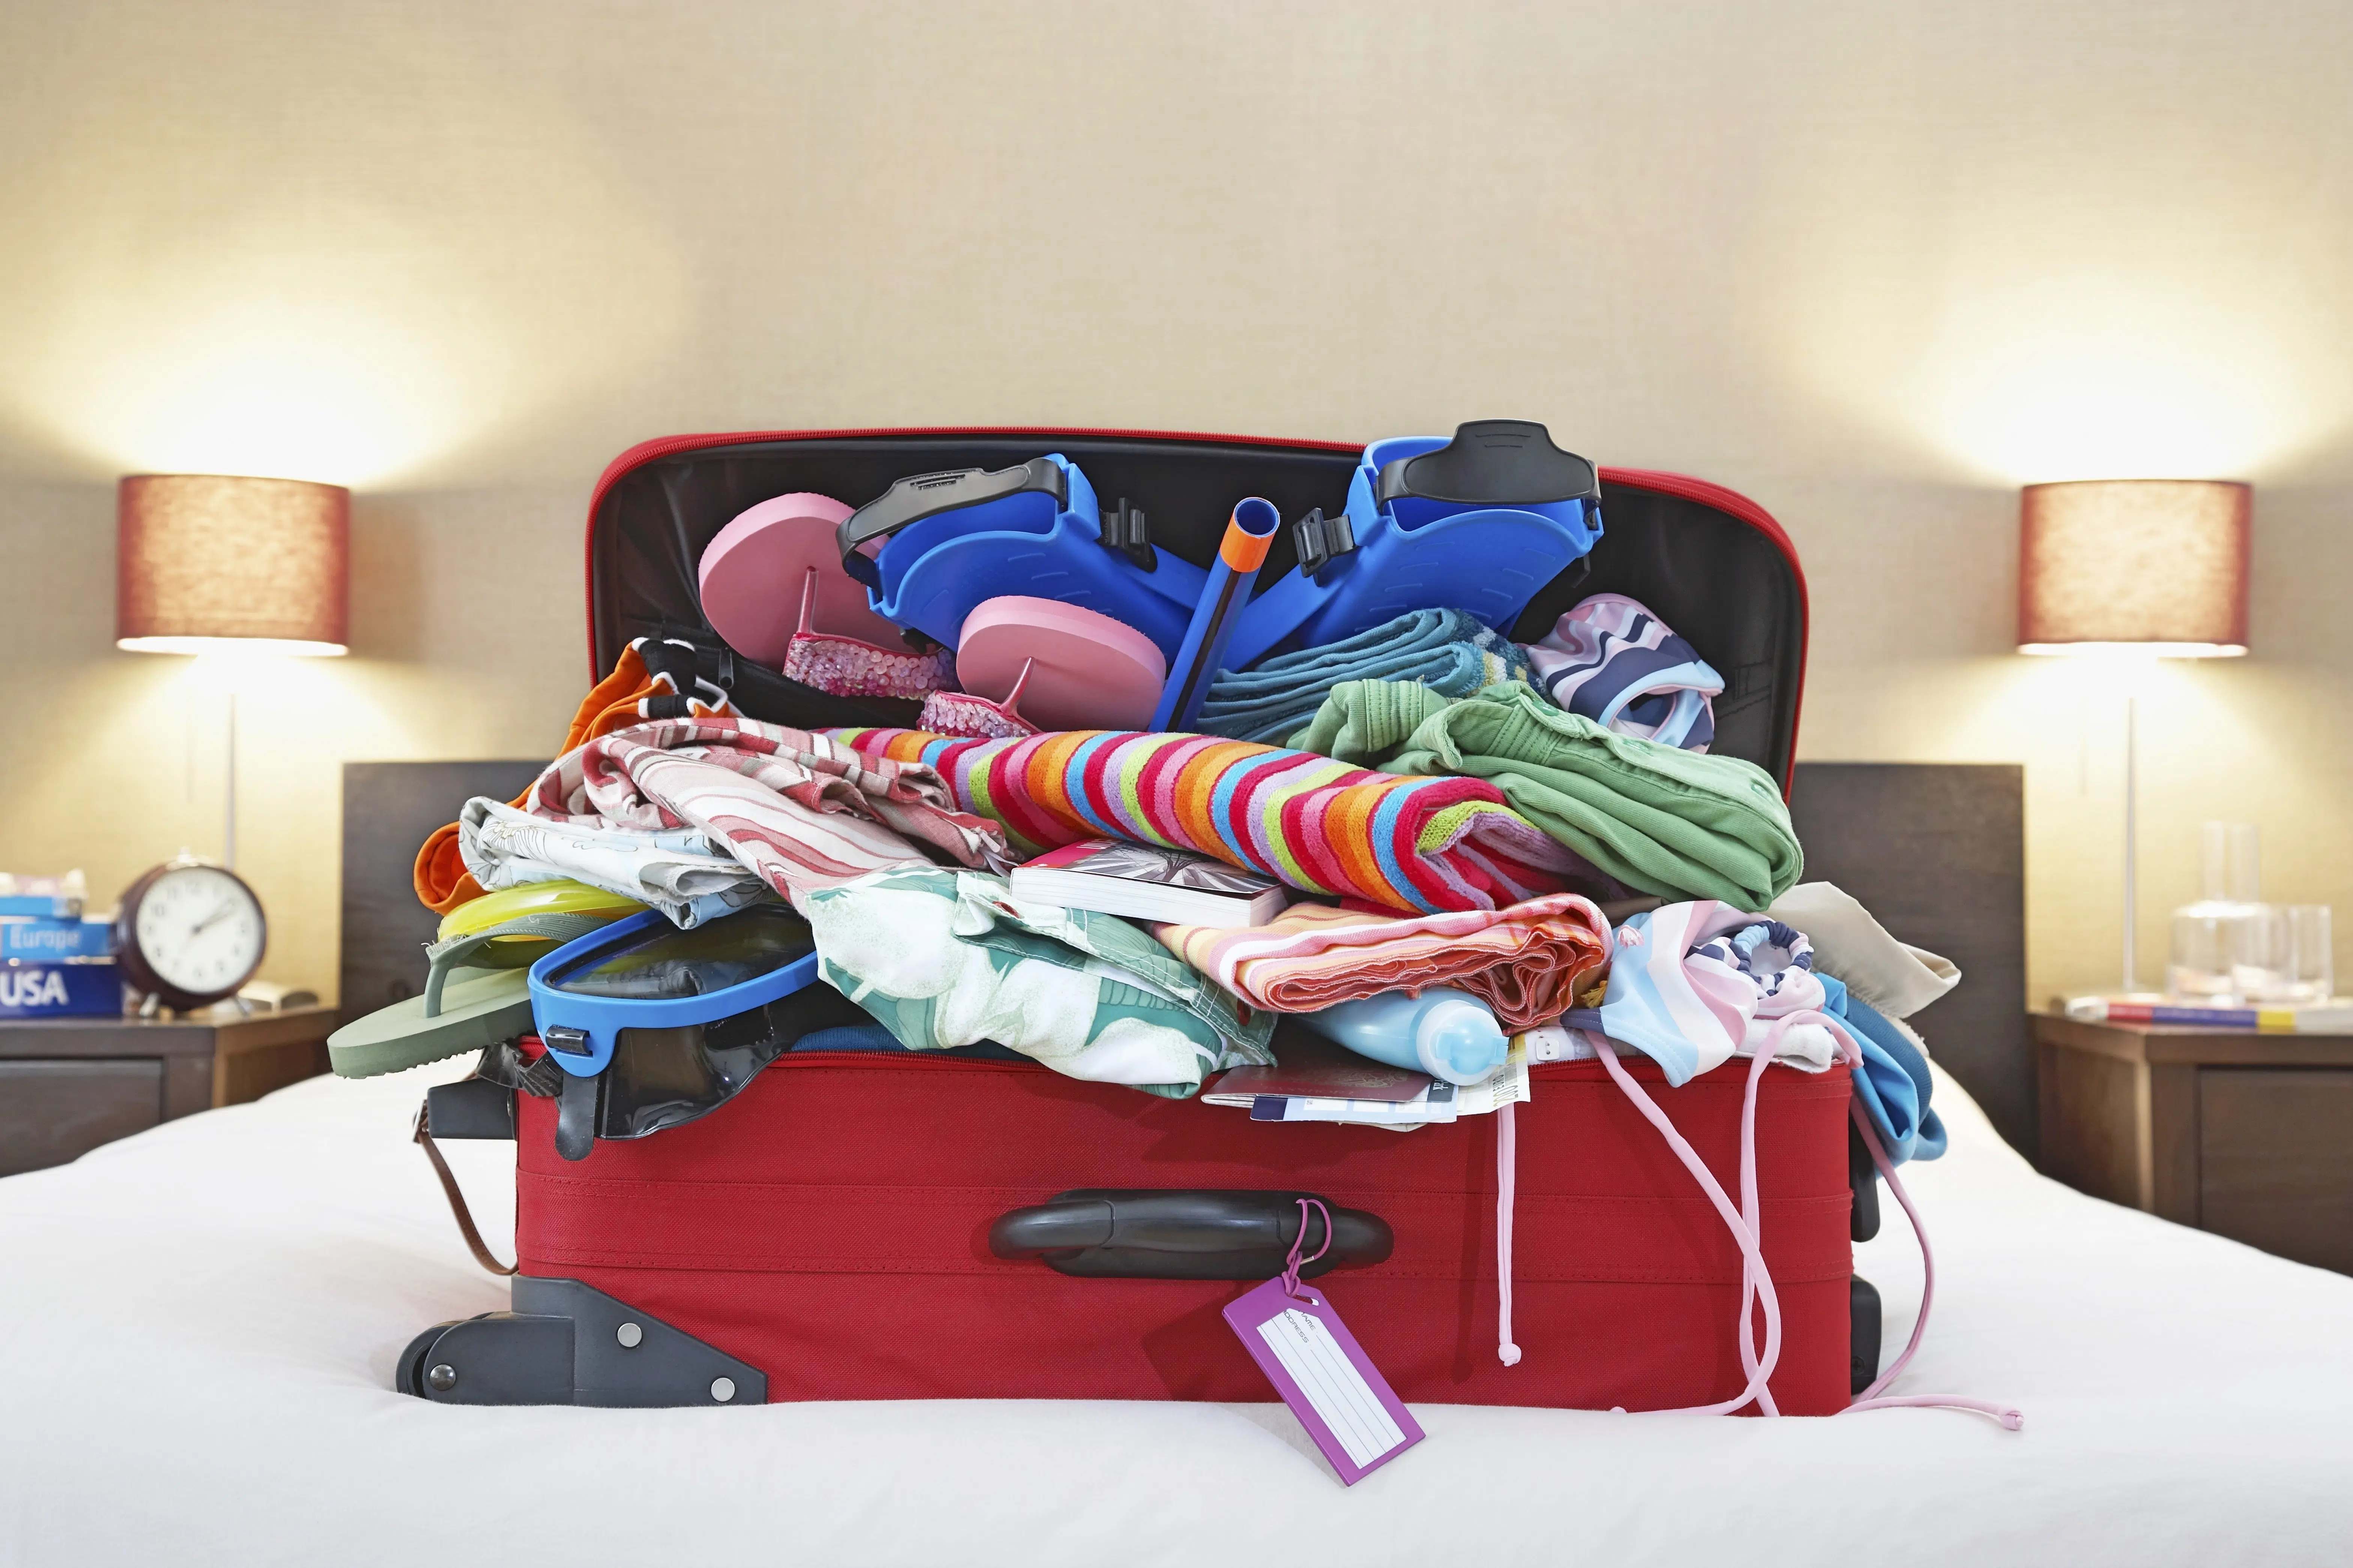
\includegraphics[width=.45\textwidth]{GrundlagenInfo/DataScience/04_Kompression/Figures/messy_suitcase.jpg}}
		\raisebox{-0.5\height}{$\rightarrow$}
		\raisebox{-0.5\height}{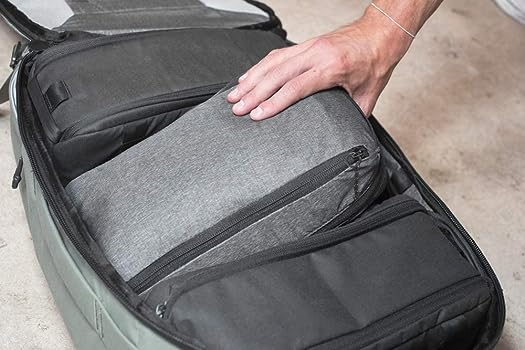
\includegraphics[width=.45\textwidth]{GrundlagenInfo/Programmieren/Figures/prog-packing-cubes}}
	\end{figure}
\end{frame}

\begin{frame}{Weshalb Kompression? \emoji{clamp}}
	\begin{itemize}
		\item Speicherplatz optimieren
	\end{itemize}
	\begin{figure}[H]
		\centering
		\raisebox{-0.5\height}{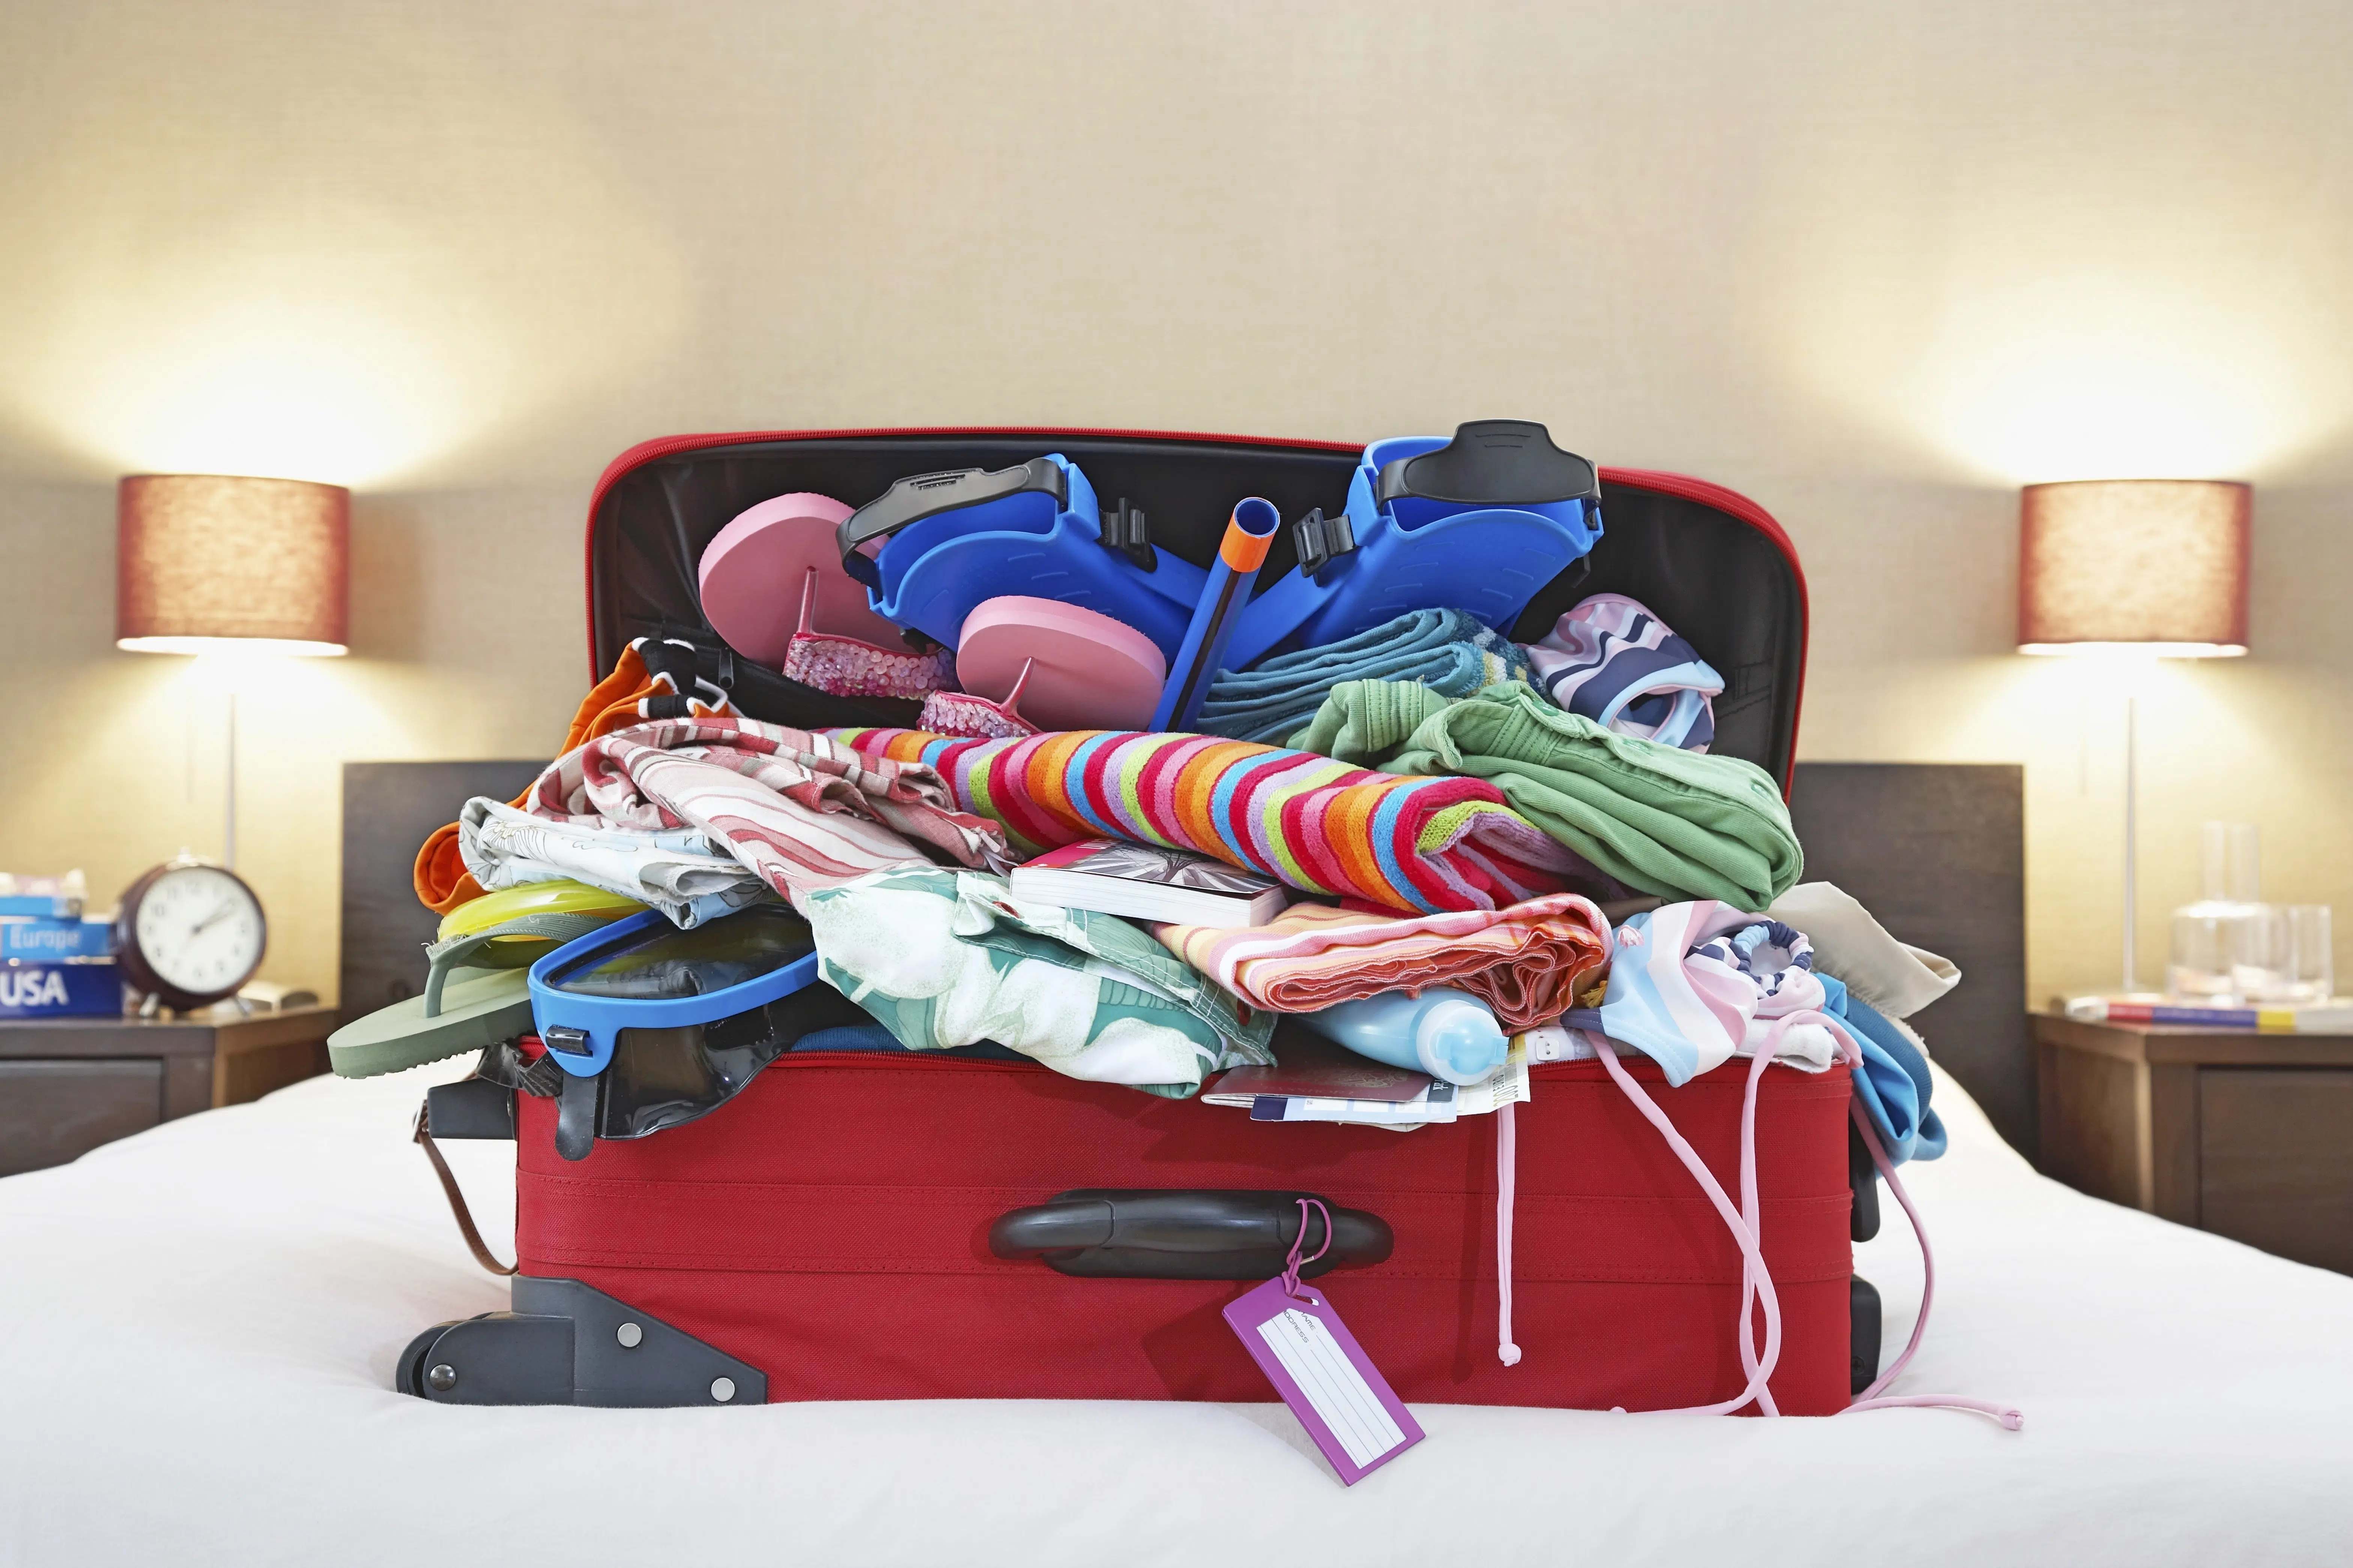
\includegraphics[width=.45\textwidth]{GrundlagenInfo/DataScience/04_Kompression/Figures/messy_suitcase.jpg}}
		\raisebox{-0.5\height}{$\rightarrow$}
		\raisebox{-0.5\height}{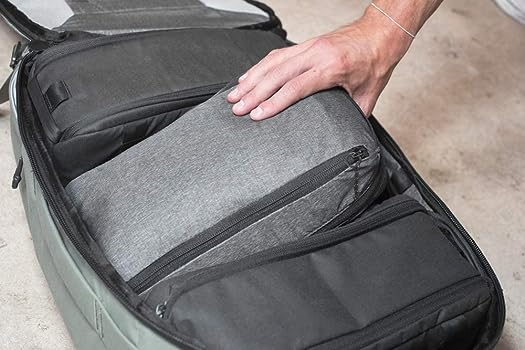
\includegraphics[width=.45\textwidth]{GrundlagenInfo/Programmieren/Figures/prog-packing-cubes}}
	\end{figure}
\end{frame}

\begin{frame}{Weshalb Kompression? \emoji{clamp}}
	\begin{itemize}
		\item Wartezeit verkürzen
	\end{itemize}
	\resizebox{!}{.5\height}{%
	\begin{tikzpicture}
		\path[mindmap,concept color=black,text=white]
		node[concept] {Computer}
		[clockwise from=0]
		child[concept color=green!50!black] {
			node[concept] {Computer}
			[clockwise from=90]
			child { node[concept] {Computer} }
			child { node[concept] {Computer} }
			child { node[concept] {Computer} }
			child { node[concept] {Computer} }
		}  
		child[concept color=blue] {
			node[concept] {Computer}
			[clockwise from=-30]
			child { node[concept] {Computer} }
			child { node[concept] {Computer} }
		}
		child[concept color=red] { node[concept] {Computer} }
		child[concept color=orange] { node[concept] {Computer} };
	\end{tikzpicture}}
\end{frame}

\begin{frame}{Verlustfreie vs. verlustbehaftete Kompression}
	Einige Beispiele:
	\begin{table}[H]
		\begin{tabular}{c||c|c}
			\textbf{Anwendung} & \textbf{Verlustfrei} & \textbf{Verlustbehaftet} \\\midrule
			\textbf{Audio} & \texttt{.flac, .aac} & \texttt{.mp3}\\\hline
			\textbf{Dateien} & \texttt{.zip}, \texttt{.rar} & \texttt{-}\\\hline
			\textbf{Video} & \texttt{.raw} & \texttt{.mp4}, \texttt{.avi}, \texttt{.mov} \\\hline
			\textbf{Fotografie} & \texttt{.raw}, \texttt{.psd}, \texttt{.gif} & \texttt{.jpg}, \texttt{.png}\\
			\textbf{Grafik} & \texttt{.svg}, \texttt{.pdf}
		\end{tabular}
	\end{table}


\end{frame}
\begin{frame}{Bilder: Beispiel}
	\begin{figure}
		\centering
		\begin{subfigure}{.45\linewidth}
			\begin{tikzpicture}[boximg]
				\node[anchor=south west] (img) {
\includegraphics[width=\linewidth]{{GrundlagenInfo/DataScience/04_Kompression/Figures/LeeLogo 300 dpi.jpg}}};
				\begin{scope}[x=(img.south east),y=(img.north west)]
					\node[draw,minimum height=.3cm,minimum width=.75cm] (B1) at (0.48,0.47) {};
				\end{scope}
			\end{tikzpicture}
			\caption{}
		\end{subfigure}\\[0.5\baselineskip]
		\begin{subfigure}{\linewidth}
			\begin{tikzpicture}[boximg]
				\node (img1) {
\includegraphics[width=0.9\linewidth]{GrundlagenInfo/DataScience/04_Kompression/Figures/LeeLogo 300 dpi zoom}};
				\draw (img1.south west) rectangle (img1.north east);
			\end{tikzpicture}\hfill%
			\caption{}
		\end{subfigure}
		\begin{tikzpicture}[overlay,boximg]
			\draw (B1) -- (img1);
		\end{tikzpicture}
		\caption{\texttt{LeeLogo\textbf{.jpg} (48 KB, 300 dots per inch)}}
	\end{figure}
\end{frame}

\begin{frame}{Bilder: Beispiel}
	\begin{figure}
		\centering
		\begin{subfigure}{.45\linewidth}
			\begin{tikzpicture}[boximg]
				\node[anchor=south west] (img) {
\includegraphics[width=\linewidth]{{GrundlagenInfo/DataScience/04_Kompression/Figures/LeeLogo.pdf}}};
				\begin{scope}[x=(img.south east),y=(img.north west)]
					\node[draw,minimum height=.3cm,minimum width=.75cm] (B1) at (0.48,0.47) {};
				\end{scope}
			\end{tikzpicture}
			\caption{}
		\end{subfigure}\\[0.5\baselineskip]
		\begin{subfigure}{\linewidth}
			\begin{tikzpicture}[boximg]
				\node (img1) {
\includegraphics[width=0.9\linewidth, clip, trim=115 30 130 30]{GrundlagenInfo/DataScience/04_Kompression/Figures/LeeLogo.pdf}};
				\draw (img1.south west) rectangle (img1.north east);
			\end{tikzpicture}\hfill%
			\caption{}
		\end{subfigure}
		\begin{tikzpicture}[overlay,boximg]
			\draw (B1) -- (img1);
		\end{tikzpicture}
		\caption{\texttt{LeeLogo\textbf{.pdf}, (28 KB)}}
	\end{figure}
\end{frame}

\begin{frame}{Kompression: Beispiel}
	\centering
	WENN \emoji{blush} HINTER \emoji{blush} $\triangle$, $\triangle$ EINIGE \emoji{blush} ANDEREN \emoji{blush} NACH.
	
	\only<2>{
		\rule{\linewidth}{.5pt}\\
		\textbf{Auflösung (beispielsweise)}:\\
		WENN HUNDE HINTER HUNDEN RENNEN, RENNEN EINIGE HUNDE ANDEREN HUNDEN NACH.
		}
\end{frame}

\begin{frame}{Kompression: Beispiel}
	\centering
	WENN FLIEGEN HINTER \#2 \#1, \#1 EINIGE \#2 ANDEREN \#2 NACH.
\end{frame}